\documentclass{article}%
\usepackage[T1]{fontenc}%
\usepackage[utf8]{inputenc}%
\usepackage{lmodern}%
\usepackage{textcomp}%
\usepackage{lastpage}%
\usepackage{authblk}%
\usepackage{graphicx}%
%
\title{RNA{-}seq Analysis of Host and Viral Gene Expression Highlights Interaction between Varicella Zoster Virus and Keratinocyte Differentiation}%
\author{Jeanne Gibbs}%
\affil{Blood Transfusion Centre of Slovenia, Ljubljana, Slovenia}%
\date{01{-}01{-}2010}%
%
\begin{document}%
\normalsize%
\maketitle%
\section{Abstract}%
\label{sec:Abstract}%
Talk about the medical science of superstition. Scientists have been trying to better understand how drugs are prevented from working. Until now, they have found a sinister culprit: hormones.\newline%
Previously, the chemical reaction in the liver gave rise to the drugs to fight off cancer. Now, scientists at the University of Utah have discovered a growth barrier to drugs that play a role in TNF{-}A, a chemical that clogs up the artery walls of the liver, preventing drugs from building up. The more a patient with liver disease needs to take drugs, the more like to, or resistant, they become.\newline%
TNF{-}A, the dominant agent in the drug pipeline, becomes resistant as soon as the liver releases it because the hormone estrogen plays a role, says Kyle Kurambie, M.D., M.Sc., study co{-}author and postdoctoral fellow in the department of molecular biology and the Biomedical Engineering Program at the University of Utah School of Medicine.\newline%
Patients with TNF{-}A resistance, Kurambie says, often die within months of their last course of anti{-}TNF drugs.\newline%
The pathway at the root of this pathway may have nothing to do with the heart or the immune system, as previously thought.\newline%
Now, the scientists know the molecular structure of the growth path, which they believe could be used as a genetic test for the damaging activity of TNF{-}A inhibitors. It could be used to block these auras, which play a role in nephrology, during transplants of kidneys and pancreas, they say.

%
\subsection{Image Analysis}%
\label{subsec:ImageAnalysis}%


\begin{figure}[h!]%
\centering%
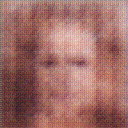
\includegraphics[width=150px]{500_fake_images/samples_5_248.png}%
\caption{A Close Up Of A Person Wearing A Suit And Tie}%
\end{figure}

%
\end{document}